\chapter{Ampliación del concepto de valor añadido}
\label{anexo:1}

El concepto valor, ha sido uno de los que ha generado mayor atención a lo largo de la relativamente corta historia del marketing, siendo abordado desde numerosas perspectivas desde los años 90 y mostrando ambigüedades conceptuales. Esto hace suponer que no se ha consensuado una definición y por lo tanto no existe una definición clara. Por todo ello, se puede afirmar que el valor es un concepto subjetivo porque cada individuo tiene diferentes perspectivas según la postura en la que se encuentre y por ese motivo, dificulta su definición (Guenzi y Troilo 2006).

Ya en el siglo IV a. C, Aristóteles dedujo que más allá de la adquisición de los bienes existía un valor propio que cada persona experimentaba a la hora de su disfrute. A este sentimiento, autores como Adam Smith o David Ricardo, destacaron la importancia del valor en el momento del intercambio de bienes, por lo que los primeros estudios del valor desde el punto de vista del marketing estarían enfocados desde esta perspectiva (Blasco, 2014).

El también conocido autor en materia económica Michael Porter (1980), da respuesta a este concepto definiendo el valor como una cadena vertical que va desde proveedores hasta clientes finales y el valor se crea a lo largo de esa cadena interviniendo los diferentes agentes del entorno. La figura \ref{fig:cincoFuerzasPorter} representa la actuación de las cinco fuerzas del mercado que interaccionan entre sí y que pueden ayudar a resolver esta cuestión.

\begin{figure}[!h]
	\caption{Las cinco fuerzas de mercado según Porter}
	\centering \includegraphics[width=130mm]{capitulos/graficos/cincoFuerzasPorter}
	\label{fig:cincoFuerzasPorter}

		\footnotesize
		Fuente: Porter, 1980
\end{figure}

En la actualidad y según la Real Academia de la Lengua Española, \emph{valor es el grado de utilidad o aptitud de las cosas, para satisfacer las necesidades o proporcionar bienestar o deleite}, pero se quiere responder cuál es el valor en el contexto de los negocios. Para el autor Sawhney (2006), el valor viene establecido por el valor percibido de un producto o servicio en relación con el coste total que los clientes pagan por el. La definición de valor por parte de la American Marketing Association (AMA 2007), expresa que el valor hay que enfocarlo desde un punto de vista de las transacciones y poniendo énfasis en el marketing como una actividad, institución y proceso por el que se pretende crear, comunicar, distribuir e intercambiar ofertas que tienen valor para clientes, socios o sociedad general. En la figura \ref{fig:cadenaAgentesPorter} se puede apreciar un pequeño modelo de esta cadena de agentes principales.

\begin{figure}[!h]
	\caption{Cadena de agentes}
	\centering 
\includegraphics[width=150mm]{capitulos/graficos/cadenaAgentesPorter}
	\label{fig:cadenaAgentesPorter}

		\footnotesize
		Fuente: Brandenburguer y Harbone, 1996, p. 9.
\end{figure}



Por otro lado, el valor influye a la hora de llevar a cabo transacciones donde también se encuentran involucrados múltiples agentes de toda la cadena productiva y comercial, como son los proveedores, las empresas, los vendedores y como no, los clientes.  

En este sentido, el valor añadido se puede definir como el valor creado a lo largo del proceso, es decir, desde el vendedor hasta el consumidor, teniendo en cuenta la cantidad y el precio que están dispuestos a invertir en un producto o servicio que no sólo cubra las necesidades, si no también que aporte algún factor añadido (Brandenburguer y Harbone, 1996). La cadena de valor se puede representar verticalmente haciendo un recorrido por las acciones que desempeñan el comprador, la empresa y el proveedor. La parte inferior de la figura \ref{fig:cadenaValor}, representa la cantidad de valor que prosee el proveedor. En la parte central se encuentra el valor adquirido por la empresa, es decir, el precio recibido por el comprador menos el coste de los recursos por parte del proveedor. En la parte superior se representa la cantidad máxima que el comprador está dispuesto a pagar por un producto o servicio. El resultado que obtenga cada agente variará dependiendo de las armas con las que se lleven a cabo las negociaciones entre los compradores y la empresa; y entre la empresa y el proveedor. Algunos de estos elementos negociadores pueden ser la persistencia, las presiones o la paciencia.

\begin{figure}[!h]
	\caption{Cadena de valor}
	\centering 
\includegraphics[width=150mm]{capitulos/graficos/cadenaValor}
	\label{fig:cadenaValor}

		\footnotesize
		Fuente: Brandenburguer y Harbone, 1996, p. 10
\end{figure}

Desde un punto de vista comercial, crear valor significa ofrecer algo a alguien que desea cubrir una necesidad y espera satisfacerla a cambio de un coste que generalmente es económico (Viscarri, 2011). Al mismo tiempo, este autor reflexiona que para las empresas cada vez es más complicado atender a todas las necesidades requeridas por los clientes ya que los mercados son cada vez más rigurosos y el entorno es cada vez más turbulento y sujeto a grandes presiones competitivas, legales, sociales y económicas. Para hacer frente a esta serie de sucesos son necesarios el esfuerzo y la integridad. Esfuerzo para mejorar e integridad para aproximarse a lo que el cliente espera, pero sin fraudes.

Sawhney (2003) establece siete fundamentos imprescindibles sobre el concepto de valor:

\begin{enumerate}
	\item \emph{El valor tiene que estar definido por el cliente}. Para Drucker (1993) lo más trascendente es lo que el cliente siente y piensa a la hora de comprar o disfrutar un bien o servicio, es decir, lo que para él tiene valor, restándose así importancia a lo que la empresa cree que tiene valor.
	\item \emph {El valor es opaco}. Las empresas tienen que realizar un ejercicio de empatía con los clientes, para poder “caminar en sus zapatos y sentir su dolor” (Drucker, 1993) (ver figura \ref{fig:empatiaMaegias}).
	\begin{figure}[!h]
	\caption{Mapa de empatía}
	\centering \includegraphics[width=110mm]{capitulos/graficos/empatiaMaegias}
	\label{fig:empatiaMaegias}

		\footnotesize
		Fuente: Megias, 2012
\end{figure}
	\item \emph {El valor es contextual}. El valor, se encuentra en los ojos, en las mentes y en los corazones de los clientes. Por lo tanto, es irrelevante hablar sobre el valor de un producto sin conocer el contexto en el que se desenvuelve la acción y sin tener en cuenta que los clientes son heterogéneos. El contexto tiene tres dimensiones importantes: el usuario final, la situación de uso final, y el medio ambiente (Drucker 1993).
	\item \emph {El valor es multidimensional} (Sawhney 2003; Lapierre, 2000):
		\begin{itemize}
			\item \emph{La dimensión funcional}. Es el valor de las características y funciones de un producto o servicio.
			\item \emph{La dimensión emocional}. Son los beneficios psicológicos que obtiene el cliente al comprar, usar, poseer o disfrutar el producto o servicio.
			\item  \emph{La dimensión económica}. Los clientes también evalúan el valor económico.

		\end{itemize}
	\item \emph{El valor es un trade-off}. Tras la lectura comprensiva de tres diccionarios monolingües\footnote{Merriam Webster, Oxford y Webster´s New World College Dictionary.}, se puede decir que trade-off es un tipo de intercambio de un producto o servicio donde el cliente le asigna un valor y lo intercambia por otro producto o servicio que valora en mayor medida. Por lo que se puede afirmar que valor es un trade-off entre el total de los beneficios que el cliente recibe y los costes totales en que incurre.
	\item \emph{El valor es relativo}. Antes de adquirir el producto o servicio, los clientes realizan una comparación entre toda la oferta de las diferentes compañías. Normalmente va a existir una alternativa a la empresa nodal\footnote{Compañía principal a estudiar o analizar.} a la que se le denomina el mejor sustituto disponible o equivalente (Sawhney, 2006), es decir, la opción que los usuarios elegirán si deciden prescindir de los servicios de esta compañía nodal
	\item \emph{El valor es un estado mental}. Para llevar a cabo una gestión basada en el valor hay que evaluar el modo de pensar de los clientes.

\end{enumerate}

Pese a que los autores no coinciden en numerosos aspectos, parece existir un consenso en que cuanta mayor intensidad tenga el papel del cliente en la creación de valor, mayor competitividad adquiere la empresa. A este marco de referencia de creación de valor conjunta se le ha denominado “co-creación de valor” (Vargo y Lusch, 2004).


\chapter{La co-creación de valor positiva o negativa para la empresa}
\label{anexo:2}

\section{El concepto de co-creación de valor positivo y negativo}

Según la teoría de Prahalad y Ramaswamy (2004), el valor se crea cuando los usuarios tienen una experiencia acumulada que viene proporcionada a través de los recursos, procesos y estados propuestos por la empresa y establecen así sus propios resultados. Dando como resultado, que el valor se realiza a través de la posesión, uso, o estados mentales del usuario. En este sentido la empresa deberá facilitar la co-creación de valor a los clientes y eso significa que la empresa ha de crear un valor potencial que el cliente puede transformar en el valor en uso o valor real. Retomando al autor Grönroos (2008), la co-creación de valor a través de la interacción en el consumo, hace que el cliente tenga sentimientos positivos, es decir, se siente mejor; o por el contrario sentimientos negativos, es decir, se siente peor. De este modo, surge la co-creación positiva o negativa con sus respectivas consecuencias para la empresa.

Aunque el concepto de experiencia acumulada de Prahalad y Ramaswamy, parece implicar un nivel constante de evolución positiva del valor, esto no ocurre en todos los casos. El proceso de acumulación de valor puede incluir tanto las experiencias positivas como las experiencias negativas de valor, donde a veces el cliente también puede llegar a ser un enemigo empresarial.

Para poder apreciar la diferencia entre una co-creación de valor positiva y negativa con más claridad, se van a exponer dos breves ejemplos prácticos. El primero de ellos es la empresa Hyve AG y la segunda es SPAR Austria.

\subsection{La co-creación de valor positiva}

Hyve AG es una conocida empresa de innovación con sede en Alemania. Su director, el Dr. Johann Fuller, afirma que el conocimiento acumulado y la creatividad, son el resultado de la interacción entre la empresa y el cliente y lo utilizan como un acelerador hacia la innovación, la mejora de la calidad del servicio y el refuerzo a la hora de retener clientes y fidelizarlos. Como consecuencia, también se puede conseguir una reducción de costes al largo plazo. La opinión de Fuller es que las empresas por si solas no pueden ofrecer propuestas de valor, y que por lo tanto son los consumidores los que crean el valor a través del uso y la aceptación del producto o servicio (Gebauer, Füller y Pezzei. 2012).

Hyve AG, ha desarrollado una plataforma Web\footnote{Hyve AG. (2015). HYVE Science Labs. Recuperado de \url{https://www.hyvescience.net/}} donde se realiza un intercambio de información entre la empresa y los usuarios. En esa página Web, la empresa comunica a los clientes las necesidades, los problemas y los retos a los que se están enfrentando. También proponen la participación de los usuarios en los proyectos. De esta forma, la empresa puede evaluar constantemente la relación del consumidor con sus productos para poder mejorar y personalizar los métodos ayudándoles a crecer como empresa y como comunidad. Por lo tanto, esta interacción se puede considerar positiva para la empresa.

\subsection{La co-creación de valor negativa}

La empresa SPAR Austria, una de las principales cadenas de distribución en Austria, creó un concurso llamado “SPAR Bag Design Contest”, traducido al castellano es “Concurso de bolsas de diseño SPAR”. Se trataba de un concurso internacional de diseño de bolsas de compra a través de la página Web del propio supermercado SPAR. El concurso invitaba a los aficionados al arte, estudiantes de diseño, diseñadores profesionales, etc. a presentar sus ideas mediante un programa informático añadido en su página Web\footnote{SPAR Österreich - Startpage. (2011). Recuperado de http://www.spar.at/de\_AT/index.html} y de fácil uso.

Tras la proclamación del ganador, la empresa tuvo que lidiar con el sentimiento de descontento de los usuarios que arremetieron contra la marca SPAR mediante quejas escritas en la página Web y comentarios negativos sobre los diseños ganadores. De este modo, los usuarios transformaron la página Web en una plataforma para expresar sus protestas. La razón principal del descontento era la decepción de los concursantes con el ganador elegido por el jurado. Se había elegido como ganador un diseño poco creativo en cuanto al diseño gráfico, pero muy ocurrente por su juego de palabras. De este modo, los participantes que no hablaban alemán no pudieron comprender ese juego de palabras. Aun así, estas reacciones negativas, proporcionaron información valiosa para SPAR sobre los factores desencadenantes de esta conducta por parte de los usuarios en las comunidades Web de innovación (Gebauer, Füller y Pezzei 2012).

Se puede afirmar, que si las expectativas del cliente no se cumplen, no surgirá el bienestar. De esta forma, la experiencia de consumo va acompañada de un efecto negativo que conduce a emociones como la ira, la frustración o la irritación. El comportamiento negativo de los consumidores puede desembocar en una conducta disfuncional de los clientes, término que se refiere a un comportamiento desviado por los clientes (Gebauer, Füller y Pezzei 2012). Los usuarios que intervienen de forma disfuncional, pueden causar serios problemas a la empresa, a los empleados e incluso a otros clientes. Esta conducta puede darse por motivos económicos, de situación o personales. Esta insatisfacción puede verse reflejada en un comportamiento de queja, realizar un boicot a la marca, actuar de manera fraudulenta o también puede que el cliente quiera sacar provecho haciendo una reclamación para recuperar un servicio gratuitamente. También es posible que se de abuso verbal o incluso físico a los empleados. Además los consumidores insatisfechos y que a su parecer no han recibido un trato justo por la empresa, también pueden llegar a ser clientes insatisfechos y activos realizando daño a la empresa mediante el boca a boca (WOM) negativo.

Pueden surgir también comunidades anti-marca. Existen multitud de éstas centradas en cuestiones ecológicas, ambientales, de derechos humanos, etc. Uno de los casos más llamativos es el que estudiaron los autores Thompson, Rindfleisch y Arsel (2006). Investigaron un fenómeno llamado el efecto Doppelgänger. Se trata de un término alemán que se usa para definir al doble fantasmagórico de una persona o cosa. En el caso de la figura \ref{fig:Starbucks}, lo que pretendía la organización de consumidores orgánicos era burlarse y poner en entre dicho a la marca Starbucks con el fin de perjudicar a la firma y ponerla en el punto de mira.

\begin{figure}[!h]
	\caption{Doppelgänger Starbucks}
	\centering 
\includegraphics[width=110mm]{capitulos/graficos/Starbucks}
	\label{fig:Starbucks}

		\footnotesize
		Fuente: adaptado de organicconsumers.org
\end{figure}

A modo resumen, se puede afirmar que no siempre las empresas consiguen los objetivos y el enfoque que pretendían en un principio con las medidas de co-creación de valor que diseñaron. No por ello, tienen que dejar de intentar co-crear valor, deberán reinventarse y seguir investigando otras vías que faciliten estos procesos de co-creación. En cuanto a la co-creación positiva, hay que señalar que el desarrollo de las nuevas tecnologías, de las Web 2.0 y de las plataformas engagement, ha favorecido la comunicación y el diálogo entre empresas y consumidores acercándoles cada vez más y ha facilitado la co-creación de valor.

\chapter{Ampliación del epígrafe \ref{section:procesosCocreacion}}
\label{anexo:3}

\section{El desarrollo de nuevos productos y/o servicios}
\subsection*{Los procesos de co-creación de valor como una oportunidad de desarrollo de nuevos productos y/o servicios}


Con este anexo, se quiere ofrecer una visión sobre el marco de actividades de co-creación de valor en los procesos de innovación empresariales. Este hecho implica la necesidad de pensar en la co-creación como un programa estratégico y no como un justo a tiempo de la externalización de las tareas de innovación (O'Hern y Rindfleisch, 2010).

Una de las características que hay que destacar del entorno de la innovación, es el reciente aumento en el contenido generado por el usuario, (CGU) y que está transformando radicalmente el panorama del marketing (Instituto de ciencia de marketing, 2008). O'Hern y Rindfleisch (2010), definen el contenido generado por el usuario como la contribución original que los usuarios aportan sobre un producto dirigido a otros usuarios, y/o el desarrollo de estos productos. Estas contribuciones proporcionan a los desarrolladores de productos de las empresas información valiosa sobre sobre el funcionamiento de un producto, cómo se puede mejorar, e incluso pueden aportar soluciones reales a los problemas relacionados con el producto.

En la actualidad es común encontrarse con un número creciente de consumidores muy bien informados y conectados y que ya no se contentan con la simple elección y uso de los productos y servicios de una empresa, sino que ellos también quieren contribuir al desarrollo y promoción de estos procesos. En los últimos años, un número creciente de académicos han comenzado a investigar el impacto del CGU en diversos campos del marketing (Chevalier y Mayzlin 2006; Godes y Mayzlin 2004), sugiriendo que el poder del CGU radica en su capacidad para llamar la atención sobre un producto y su promoción a través del boca a boca. Este término se concentra en la comunicación establecida entre consumidor y consumidor y considera al CGU como un vehículo para la promoción del producto (Godes y Mayzlin, 2004).

Retomando la teoría de O'Hern y Rindfleisch (2010), acerca de la investigación de innovación por parte del usuario, estos autores reconocen el papel activo que los usuarios adquieren en el proceso de co-creación considerándoles agentes de innovación. Un ejemplo antiguo pero claro es el de Raymond (1999) sobre los inicios de Linux. En esta empresa, tuvieron en cuenta los amplios conocimientos de sus usuarios para crear el código fuente de Linux y cuando los propios clientes encontraban fallos, los reportaban y propiciaban cambios que daban lugar a mejoras importantes. Por lo que, la innovación por parte del usuario crea contribuciones potenciales, nuevas ideas y soluciones.

Bartl (2006), establece un plan de acción a la hora de co-crear valor en productos o servicios innovadores, dando respuesta a cuándo, quién y cómo co-crear.

En lo que se refiere a la primera cuestión, Michael Bartl (2009) parte de la división del proceso de innovación en cinco fases:

\begin{enumerate}
	\item \emph{Oportunidades e ideas}.
	\item \emph{Conceptos}.
	\item \emph{El diseño y la ingeniería}.
	\item \emph{Pruebas}.
	\item \emph{Lanzamiento}.
\end{enumerate}

Normalmente, las empresas a la hora de co-crear centran principalmente sus objetivos en la participación de los clientes finales, consumidores o usuarios. Sin embargo, en algunos casos también se deberían de tener en cuenta a otros grupos de intermediarios como clientes corporativos, distribuidores, socios comerciales, instituciones gubernamentales o las asociaciones de consumidores. La duración y la estabilidad de la relación con el cliente depende de una diferenciación entre los clientes existentes, los latentes y los nuevos.

El desarrollo de las TIC, ha propiciado herramientas diseñadas para el cliente online. Un número cada vez mayor de usuarios están contribuyendo activamente a la creación de ideas y a proporcionar soluciones online. Estos usuarios online juegan un papel muy importante para las empresas porque expresan sus propias percepciones de la calidad del producto. En el caso de los clientes fieles, incluso pueden influir en las actividades de promoción de la competencia de la empresa realizando comentarios de desprestigio (Mayzlin, 2006). Un ejemplo es la campaña de XS desprestigiando la bebida austríaca Red Bull\footnote{Tejada, M, C. (2015). El nuevo diario. Recuperado de www.elnuevodiario.com.do/mobile/article.aspx?id=17531}.

Una de las cuestiones importantes de la co-creación de valor es establecer en qué etapa del proceso de innovación los clientes pueden tener una mayor participación, bien en la generación de ideas, en la evaluación y refinamiento de conceptos, en especificar las características del producto o en la creación de prototipos, etc. Por lo tanto, se puede decir que el consumidor puede ser de utilidad creativa influyendo en las tres primeras fases de Bart (2006), es decir, creando oportunidades e ideas, concretándolas y participando en el diseño o incluso en la ingeniería. Un ejemplo, son las páginas Web Dell IdeaStorm\footnote{Dell Idea Storm. (2015). Recuperado de www.ideastorm.com/} o Lego\footnote{LEGO.com Digital Designer Virtual Building Software. (2015). Recuperado de http://ldd.lego.com/en-us/}. Estas páginas Web se utilizan como un medio de comunicación entre los consumidores y los desarrolladores y se consideran como un mecanismo en el que los consumidores aportan ideas y soluciones que pueden influir directamente en la innovación de productos (O'Hern y Rindfleisch, 2010). Por otro lado, se encuentran los procesos por los que las empresas tienen un producto ya desarrollado y lo que pretenden es innovar a partir de ese producto base, como es el caso de BMW\footnote{Bilgram,V. (2010). Value Co-Creation: From Piloting to Continuous Co-Creation. Recuperado de http://value-co-creation.blogspot.co.at/2010/11/from-piloting-to-continuous-co-creation.html} y Nivea\footnote{Bilgram,V. (2011). Nivea's Co-Creation Process: the Case of the Invisible for Black \& White. Recuperado de http://www.slideshare.net/HYVE/2011-0228-nivea-invisible-for-black-white-deodorant}. En estos casos, el proceso de co-creación surge en las últimas etapas descritas por Bartl (2009), es decir, en los test y puesta en marcha del producto o servicio.

Otra idea que hay que señalar de Bartl (2009), es el grado de implicación de los usuarios para que participen en las actividades propuestas de co-creación. Hay dos vertientes:

\begin{enumerate}
	\item \emph{La motivación intrínseca}.
	\item \emph{La motivación extrínseca}.
\end{enumerate}

La motivación intrínseca de los clientes es el hecho de realizar una acción para satisfacer una necesidad y sentirse motivado al llevarla a cabo por un aspecto separable, es decir, cuando una persona se encuentra motivada intrínsecamente, actúa con una finalidad lúdica y no suele encontrarse motivada por agentes externos, o por sentirse presionada o por una posible recompensa futura. En cambio, la motivación extrínseca se da cuando el consumidor se ve motivado por las recompensas externas, bien sean intereses económicos, o recompensas. (Ryan y Deci, 2000). Para poder comprender estos dos términos, se van a citar algunos ejemplos. La motivación intrínseca es palpable en los niños pequeños porque tratan constantemente de agarrar, tirar, morder o gritar a los objetos nuevos que se encuentran para poder obtener información de ellos. A medida que estos niños van creciendo, el entorno les hace seguir estando intrínsecamente motivados a través de crucigramas, de la lectura de novelas o incluso del hecho de ver películas. Por otro lado, algunos casos de la motivación extrínseca pueden llevarse a cabo mediante recompensas externas, como por ejemplo dinero o ascensos en los puestos de trabajo (Bartl 2009).

Retomando el caso de los consumidores, los usuarios que estén motivados intrínsecamente valorarán el intercambio comercial de una forma muy intensa, sin embargo, si están motivados extrínsecamente sólo se centrarán en los resultados. Por lo tanto, algunas de las motivaciones intrínsecas que puede tener el consumidor son: la curiosidad, la auto eficacia, el desarrollo de actividades, la búsqueda de información, la necesidad personal, etc. La motivación intrínseca destaca en los clientes altamente involucrados y que ayudan en mayor medida al proceso de co-creación de valor. No obstante, cuando las empresas buscan co-crear con los usuarios en productos innovadores, la motivación deberá ser intrínseca y extrínseca, ya que tienen que tienen que exponer el 100\% de sus ideas teniendo en cuenta sus motivaciones y manifestar los resultados finales que quieren obtener.

Por lo tanto, un programa de co-creación de valor en productos innovadores, debe estar caracterizado por una relación de colaboración continua entre la empresa y los usuarios. Esta relación se describe de una forma gráfica en la figura \ref{fig:cocreacionInnovacionBartl}. Las interacciones entre la compañía y los clientes deben darse a lo largo del proceso de innovación y las ideas que se desarrollen tienen que concordar con los límites y los resultados de la organización.

\begin{figure}[!h]
	\caption{Enfoque programático para la formación de co-creación continua}
	\centering \includegraphics[width=140mm]{capitulos/graficos/cocreacionInnovacionBartl}
	\label{fig:cocreacionInnovacionBartl}

		\footnotesize
		Fuente: Bartl, 2010
\end{figure}

Como se puede apreciar en la figura \ref{fig:cocreacionInnovacionBartl}, pueden existir diferentes procesos de co-creación, representados con los círculos en forma de flechas, en un mismo momento del desarrollo del producto. Las flechas indican la necesidad no sólo de buscar y adquirir innovación, sino también asimilar y explotar esta entrada dentro de todos los procesos siguientes.

A su vez, estos procesos co-creativos de innovación pueden estar más o menos abiertos, representados a través de los diferentes tonos de grises. Cuanta mayor intensidad tenga el tono gris, querrá decir que ese proceso de co-creación es cerrado. Un ejemplo de ello pueden ser los blogs que facilitan las actualizaciones del proyecto, la organización, la comunicación con el cliente, etc. También, las redes sociales pueden proporcionar recursos desconocidos, mayor accesibilidad de los clientes a la empresa, datos de contacto, etc. Ambos forman parte de una amplia lista de elementos de un proceso cerrado de co-creación y es una forma rápida de conectar las opiniones y las visiones de los consumidores con la empresa. En cambio, cuanto menor intensidad tenga el color gris, el proceso de co-creación es más abierto, lo que supone que los clientes se involucren en mayor medida. Por ejemplo, en el año 2006 los fans de Doritos diseñaron sus propios anuncios para tener la oportunidad de ganar un viaje para ver en directo la Super Bowl. Otro ejemplo, como se ha señalado anteriormente, es la empresa Lego que cuenta con un sitio web donde invita a desarrollar ideas y proyectos a sus seguidores con la opción de poder fabricarlos en un futuro. La empresa también tiene que ser consciente de que los usuarios han de adaptarse a las herramientas que ésta les proporciona y de delimitar los límites hasta los que pueden involucrarse en el proceso de la co-creación, o por el contrario indicar a sus consumidores que no existen límites porque el proceso de co-creación es totalmente abierto. Por ejemplo, los círculos más cerrados, los grises, pueden ser herramientas enterprise 2.0; y los círculos más abiertos, los blancos, pueden ser plataformas crowdsourcing.

Para poder comprender estos términos, se ha de mencionar en primer lugar que el concepto de Web 2.0 y sus dinámicas de funcionamiento, hacen que se desemboque en el concepto de enterprise 2.0. Enterprise 2.0 es a la utilización por parte de las empresas, clientes y socios, del uso de plataformas software para la difusión de noticias, concursos, experiencias, etc. Las empresas que proponen este tipo de software a disposición de sus clientes, han sufrido una modificación de valores empresariales porque consideran a estas plataformas como software social, ya que disponen de las características y las funciones necesarias para cubrir las necesidades de la sociedad. Algunos ejemplos de entidades que utilizan estas herramientas para crear contenido son Flickr, Google, Wikipedia, etc (Forbes, 2010). Por otro lado, las plataformas Crowdsourcing son un nuevo modelo de negocio que se utiliza para externalizar de forma distribuida las tareas de la empresa. También se utiliza para poder crear ideas y solucionar problemas comunes entre todos los agentes.

\begin{figure}[!h]
	\caption{La co-creación en proyectos de innovación}
	\centering 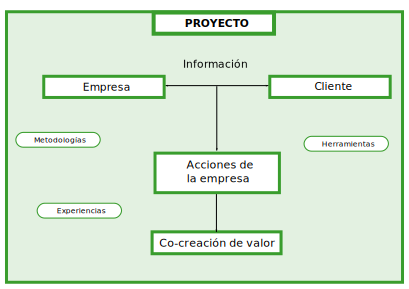
\includegraphics[width=140mm]{capitulos/graficos/proyectoInnovacionBartl}
	\label{fig:proyectoInnovacionBartl}

		\footnotesize
		Fuente: adaptado de Bartl, 2009
\end{figure}

Con todo lo explicado anteriormente, se puede decir que el éxito de la co-creación en proyectos de innovación depende de tres factores fundamentales (ver figura \ref{fig:proyectoInnovacionBartl}). En primer lugar, la excelencia del proyecto en términos metodológicos, las herramientas y las experiencias que la empresa debe de cumplir. En segundo lugar, diseñar un proceso de co-creación de valor continuo, creando un proceso interactivo entre los consumidores y la empresa. Y por último, las estructuras y las capacidades de la organización que tienen que establecerse con el fin de no ser sólo informaciones que den los usuarios si no que tengan como finalidad llevar a cabo mejores productos orientados hacia el cliente y aprovechar la co-creación de valor dentro de la empresa (Bartl, 2009).


\chapter{Ampliación del epígrafe \ref{section:logicasDominantes}}
\label{anexo:4}

\section{De la lógica dominante del producto a la lógica dominante del servicio}

Cómo se ha podido observar en la figura \ref{fig:evolucion} del capítulo \ref{section:cocreacion}, en 1960 nacen tres nuevos enfoques surgidos de la LDP (Vargo y Lusch, 2008):

\begin{itemize}
	\item \emph{El business to business (B2B)}. Se trata de la necesidad empresarial de abordar temas tales como el marketing industrial, la incapacidad de comercializar con ciertos productos, la incomprensión por parte de la LDP del concepto de intercambio, etc. De este modo nació el B2B.
	\item \emph{Marketing de servicios}. Cuyas diferencias básicas con la LDP son las siglas IHIP: Inseparabilidad de la producción y consumo, heterogeneidad, inventariabilidad y servicios perecederos. Por lo que las compañías tienen que ajustarse a estas diferencias. También, los investigadores comenzaron a encontrar alternativas como las relaciones en las transacciones, la calidad percibida por el cliente en lugar de tener en cuenta la marca entre otros.
	\item \emph{La teoría de la intersección}. Tiene su base en la reconceptualización del marketing, de producir bienes a producir algo más que servicios. Por ejemplo, en aerolíneas, bancos, salud, hoteles, etc., se ha de cambiar el concepto de producción de unidades de servicios a producir servicio. Vargo y Lusch (2008) afirman que el surgimiento de la LDS surge de esta rama.
\end{itemize}

\chapter{Aplicación de la lógica del servicio}
\label{anexo:5}

A continuación se exponen los 11 puntos que Grönroos (2006) ha desarrollado acerca de la lógica del servicio y su postura hacia el autoservicio.


\section{Las proposiciones de Grönroos (2006) relacionadas con la creación de valor y el autoservicio:}

\begin{itemize}
	\item La LS apoya la creación de valor para los clientes por sí solos mediante el autoservicio.
	\item En el autoservicio también se puede co-crear valor. Los bienes y servicios han sido adquiridos por los clientes, junto con otros recursos necesarios que son utilizados por los clientes como recursos de entrada y los usuarios han de desarrollar su conocimiento y habilidad.
	\item Teniendo en cuenta el caso anterior, mediante el uso de estos recursos y la aplicación de esos conocimientos en el proceso de generación de valor en el autoservicio, los clientes van a crear valor para ellos mismos.
	\item La empresa por si sola no puede crear valor para los clientes. Su función es ser \emph{facilitadora} de valor, es decir, proporciona a los clientes los productos y servicios necesarios para facilitar los procesos de generación de valor en el autoservicio. Por lo tanto, se puede decir que la empresa está indirectamente involucrada con los clientes en la creación de valor.
	\item Y por último, otra de las funciones de la empresa, es la creación de oportunidades para desarrollar las interacciones con sus clientes durante sus procesos de generación de valor. Este hecho, provoca el cumplimiento de valor para los clientes y por lo tanto se convierten en co-creadores de valor.
\end{itemize}

\section{Las proposiciones relacionadas con la oferta del mercado:}

\begin{itemize}
	\item Ha de surgir el apoyo a los recursos, tales como bienes, servicios, información e interacciones entre el cliente y la empresa en el proceso de creación de valor de los propios clientes. La propuesta de co-creación de valor se produce gracias a la interacción entre ambos.
	\item Los clientes utilizan los bienes y servicios para producir un servicio por si solos que crea valor para ellos.
	\item La adopción de la LS es una decisión estratégica. Si los clientes no están comprando los bienes y servicios, la empresa puede persuadirlos.

\end{itemize}

\section{Las proposiciones relacionadas con el marketing:}

\begin{itemize}
	\item La aplicación de la LS significa que la empresa no se limita a hacer propuestas de valor único, sino que también recibe oportunidades. Por ejemplo, través de las posibilidades de co-creación de valor durante las interacciones con los clientes. De este modo, la empresa participa activa y directamente en la co-creación de valor para sus clientes.
	\item En la LS, la interacción en el momento del intercambio es la base de la comercialización, es decir, el cambio no se orienta hacia la creación de valor de los clientes, sino hacia las transacciones y hacia la facilitación del valor.

\end{itemize}

\chapter{Concepto de walmartización}
\label{anexo:6}

La walmartización es un concepto moderno con el que Prahalad y Ramaswamy (2004) pretenden explicar porqué las empresas han de poner todos los medios de los que disponen para que el cliente se sienta lo suficientemente cómodo a la hora del intercambio y pueda crear valor a través de la experiencia. Según el diccionario Collins, la walmartización se produce cuando una gran empresa o cadena de empresas se mueven de una región a otra y devasta/n a las empresas locales. Además, estas empresas impulsan a los trabajadores a desplazarse y a percibir una renta más baja. Por lo tanto, teniendo en cuenta este concepto, la globalización, la desregulación, la externalización y la convergencia de las industrias, y las tecnologías están haciendo que sea más difícil diferenciar las ofertas. Esto quiere decir, que los productos y los servicios se enfrentan a la mercantilización. La mercantilización se da cuando las empresas son eficientes pero los consumidores no aprecian ninguna diferencia entre si van o no a comprar de forma inteligente y barata.

\chapter{Cuestionario clientes}
\label{anexo:7}

\section*{Instrucciones}

El cuestionario consta de 36 preguntas y es de tipo mixto. Usted deberá responder con la máxima sinceridad posible y de una forma subjetiva. En cada pregunta tiene la oportunidad de exponer sus ideas, quejas o valoraciones.

El cuestionario está dividido en dos partes. La primera, es un cuestionario tipo Likert en el que deberá de elegir el número que mejor se adapte a sus experiencias vividas a lo largo de su estancia en este hotel. La escala es la siguiente:

\begin{enumerate}
	\item Muy insatisfecho.
	\item Insatisfecho.
	\item Ni satisfecho ni insatisfecho.
	\item Satisfecho.
	\item Muy satisfecho.

	\end{enumerate}
El segundo cuestionario es de tipo dicotómico en el que sólo hay dos posibilidades: si y no. A su vez, este cuestionario está subdividido en apartados.

\section*{Parte 1}
Responda desde muy insatisfecho (1) a muy satisfecho (5):

\begin{enumerate}
	\item ¿Su reserva antes de llegar al hotel fue gestionada eficientemente?
	\item ¿Cómo fue su experiencia durante el check in?
	\item ¿Cómo fue su experiencia global con la habitación?
	\item ¿Qué le pareció la cama?
	\item ¿Está satisfecho con el baño de la habitación?
	\item ¿Está satisfecho con las amenidades del baño y los productos de aseo que el hotel le proporcionó?
	\item ¿Cómo evalúa la atención al huésped en general?
	\item ¿Está satisfecho con el servicio de desayunos?
	\item ¿Cómo evalúa los servicios de Internet y WiFi en el hotel?
	\item ¿Cómo ha sido el trato recibido por parte de los empleados a lo largo del check out?
	\item ¿Cómo ha sido la actitud y proactividad de los empleados durante su estancia en el hotel?
	\item ¿Qué le pareció la atmósfera del hotel (música, aroma, iluminación, decoración, mobiliario)?
	\item ¿Le parece adecuado el plan de fidelización que propone el hotel?
	\item ¿Cómo fue su experiencia global en el hotel?
	\item ¿Sintió que le mimamos durante su estancia?
	\item Cómo evalúa la relación calidad – precio global?
	\item ¿Volverá a este hotel?
	\item ¿Recomendará este hotel?
	\item ¿Cómo evaluaría el minibar de la habitación?
	\item ¿Cómo evaluaría la tintorería y el servicio de limpieza en seco?
	\item ¿Está satisfecho con el servicio durante la comida?
	\item ¿Está satisfecho con el servicio durante la cena?
	\item ¿Cómo evaluaría su experiencia en el bar?
	\item ¿Cómo evaluaría su experiencia en el gimnasio?
	\item ¿Cómo evaluaría el servicio de habitaciones?

\end{enumerate}

\section*{Parte 2}
Responda si/no.


\subsection*{Participación}
\begin{enumerate}
	\item ¿Promueve la oferta cultural de la ciudad de Viena?
	\item ¿Proporciona usted productos y servicios sostenibles a otros huéspedes?
	\item ¿Apoya a las actividades de las ONGs o de otras organizaciones locales?
	\item ¿Administra los recursos naturales de una forma responsable (agua, energía, desperdicios)?
	\item ¿Contribuye al desarrollo económico de este hotel con su estancia?
	\item ¿Le gustaría enviar su opinión a Tripadvisor a través de esta encuesta?

\end{enumerate}

\subsection*{Problemas}
\begin{enumerate}
	\item ¿Tuvo algún problema?
	\item ¿Reportó ese problema?

\end{enumerate}

\subsection*{Fidelización}
\begin{enumerate}
	\item Durante su estancia, ¿le informaron sobre los beneficios del programa de fidelidad?
	\item ¿Es miembro del programa de fidelidad?
	\item ¿Se hizo miembro del programa de fidelidad durante la última estancia?

\end{enumerate}

Los ítems número: 19, 20, 21, 22, 23, 24 y 25 que son de tipo Likert, han sido eliminados del estudio debido a la escasez de respuestas o a la escasez de fiabilidad que aportaban según el análisis factorial realizado. Por lo tanto, el contraste de hipótesis se ha llevado a cabo con un total de 29 ítems divididos en 6 factores.

\chapter{Resultados SPSS del estudio 1. Análisis factorial}
\label{anexo:8}

\begin{table}[h]
    \caption {Prueba de KMO y Bartlett del estudio 1}
	\label{tab:kmo1}
	\setlength\extrarowheight{5pt}
	
	\begin{tabular}{p{5.7cm} p{4.6cm} p{2.8cm}}
	\toprule
	\multicolumn{2}{c}{Medida de adecuación de muestra de Kaiser-Meyer-Olkin}	& 0,611 \\
									& Chi-Cuadrado aprox	& 462,649 \\
	Test de esfericidad de Bartlett	& Desviación estándar					& 153 \\
									& Significación					& 0.000 \\
	\bottomrule
	\end{tabular}
	
	\center
	\footnotesize
	Fuente: elaboración propia
\end{table}


\begin{figure}[!h]
	\caption{Gráfico de sedimentación}
	\centering \includegraphics[width=150mm]{capitulos/graficos/sedimentacion}
	\label{fig:sedimentacion}

		\footnotesize
		Fuente: elaboración propia
\end{figure}

\newpage

\begin{table}[h]
    \caption {Varianza total explicada estudio 1}
	\label{tab:varianzaExplicada1}
	\setlength\extrarowheight{5pt}
	
	\begin{tabular}{p{1.5cm} p{1.9cm} p{1.7cm} p{1.7cm} p{1.9cm} p{1.9cm} p{1.7cm}}
	\toprule
	Comp.	& \multicolumn{3}{c}{Valores propios iniciales} & \multicolumn{3}{c}{Rotación de las sumas de los cuadrados} \\
	\midrule
		& Total	& \% de varianza	& \% acumulado	& Total	& \% de varianza 	& \% acumulado \\
	\midrule
	1  & 8,042 & 44,680 & 	44,680 & 5,059 & 28,106 & 28,106 \\
	2  & 2,285 & 12,697 & 	57,376 & 4,054 & 22,524 & 50,629 \\
	3  & 1,648 & 9,157 &	66,534 & 2,863 & 15,904 & 66,534 \\
	4  & 1,176 & 6,534 &	73,068 &  &  &  \\
	5  & 0,934 & 5,188 &	78,256 &  &  &  \\
	6  & 0,835 & 4,638 &	82,894 &  &  &  \\
	7  & 0,711 & 3,952 &	86,846 &  &  &  \\
	8  & 0,560 & 3,112 &	89,958 &  &  &  \\
	9  & 0,516 & 2,866 &	92,823 &  &  &  \\
	10 & 0,304 & 1,689 & 	94,513 &  &  &  \\
	11 & 0,259 & 1,437 & 	95,949 &  &  &  \\
	12 & 0,219 & 1,217 & 	97,166 &  &  &  \\
	13 & 0,185 & 1,028 & 	98,194 &  &  &  \\
	14 & 0,125 & 0,692 & 	98,886 &  &  &  \\
	15 & 0,110 & 0,611 & 	99,498 &  &  &  \\
	16 & 0,050 & 0,277 & 	99,775 &  &  &  \\
	17 & 0,025 & 0,138 & 	99,913 &  &  &  \\
	18 & 0,016 & 0,087 & 	100,000 &  &  &  \\
	\bottomrule
	\end{tabular}
	
	\center
	\footnotesize
	Método de extracción: Análisis del componente principal.\\
	Fuente: elaboración propia
\end{table}


\newpage

\begin{table}[h]
    \caption {Matriz de componentes rotados}
	\label{tab:componentes1}
	\setlength\extrarowheight{5pt}
	
	\begin{tabular}{p{7.0cm} p{2.3cm} p{2.3cm} p{1.5cm}}
	\toprule
		& \multicolumn{3}{c}{Componentes} \\
		& 1	& 2	& 3	\\
	\midrule
	Recomendar hotel & 0,872 &  & \\
	Desayuno & 0,812 &  & \\
	Amenidades baño & 0,762 &  & \\
	Calidad-precio & 0,722 &  & \\
	Volver hotel & 0,720 &  & \\
	Baño & 0,706 &  & \\
	Experiencia global hotel &  & 0,606 & \\
	Check in &  & 0,760 & \\
	Cama &  & 0,725 & \\
	Experiencia global habitación &  & 0,687 & \\
	Atmósfera hotel &  & 0,651 & \\
	Reserva gestionada bien &  & 0,645 & \\
	Atención al huésped &  & 0,599 & \\
	WiFi	&	& 0,458	&	\\
	Check out &  &  & 0,821 \\
	Proactividad empleados &  &  & 0,707 \\
	Mimos	&	&	&	0,615 \\
	Fidelidad	&	&	& 0,568 \\
	\bottomrule
	\end{tabular}
	
	\center
	\footnotesize
	Método de extracción: Análisis del componente principal.\\
	Método de rotación: Varimax con normalización de Kaiser.\\
	Fuente: elaboración propia
\end{table}


A continuación se muestran los nombres utilizados para nombrar a las variables en SPSS con sus respectivas preguntas.

\begin{itemize}
	\item \emph{Reserva gestionada bien.} ¿Su reserva antes de llegar al hotel fue gestionada eficientemente?
	\item \emph{Check in.} ¿Cómo fue su experiencia durante el checkin?
	\item \emph{Experiencia global habitación.} ¿Cómo fue su experiencia global con la habitación?
	\item \emph{Cama.} ¿Qué le pareció la cama?
	\item \emph{Baño.} ¿Está satisfecho con el baño de la habitación?
	\item \emph{Amenidades baño.} ¿Está satisfecho con las amenidades del baño y los productos de aseo que el hotel le proporcionó?
	\item \emph{Atención al huesped.} ¿Cómo evalúa la atención al huésped en general?
	\item \emph{Desayuno.} ¿Está satisfecho con el servicio de desayunos?
	\item \emph{WiFi.} ¿Cómo evalúa los servicios de Internet y WiFi en el hotel?
	\item \emph{Check out.} ¿Cómo ha sido el trato recibido por parte de los empleados a lo largo del check out?
	\item \emph{Proactividad empleados.} ¿Cómo ha sido la actitud y proactividad de los empleados durante su estancia en el hotel?
	\item \emph{Atmósfera hotel.} ¿Qué le pareció la atmósfera del hotel (música, aroma, iluminación, decoración, mobiliario)?
	\item \emph{Experiencia global hotel.} ¿Cómo fue su experiencia global en el hotel?
	\item \emph{Mimos.} ¿Sintió que le mimamos durante su estancia?
	\item \emph{Calidad-precio.} Cómo evalúa la relación calidad – precio global?
	\item \emph{Volver hotel.} ¿Volverá a este hotel?
	\item \emph{Recomendar hotel.} ¿Recomendará este hotel?
	\item \emph{Fidelidad.} ¿Le parece adecuado el plan de fidelización que propone el hotel?
\end{itemize}

\chapter{Resultados SPSS del estudio 1. Aceptación y fiabilidad de los factores}
\label{anexo:9}

\section{Factor co-creación}

\begin{table}[h]
    \caption {Prueba de KMO y Bartlett de la co-creación}
	\label{tab:kmo2}
	\setlength\extrarowheight{5pt}
	
	\begin{tabular}{p{5.7cm} p{4.6cm} p{2.8cm}}
	\toprule
	\multicolumn{2}{c}{Medida de adecuación de muestra de Kaiser-Meyer-Olkin}	& 0,665 \\
									& Chi-Cuadrado aprox	& 76,793 \\
	Test de esfericidad de Bartlett	& Desviación estándar					& 6 \\
									& Significación					& 0.000 \\
	\bottomrule
	\end{tabular}
	
	\center
	\footnotesize
	Fuente: elaboración propia
\end{table}


\begin{table}[h]
    \caption {Estadísticas de fiabilidad de la co-creación}
	\label{tab:fiabilidadCocreacion}
	\setlength\extrarowheight{5pt}
	
	\begin{tabular}{p{5.7cm} p{4.6cm} p{2.8cm}}
	\toprule
	Alfa de Cronbach	& Alfa de Cronbach basada en elementos estandarizados	& Nº de elementos \\
	\midrule
	0,837				& 0,852					& 6 \\
	\bottomrule
	\end{tabular}
	
	\center
	\footnotesize
	Fuente: elaboración propia
\end{table}


\begin{table}[h]
    \caption {Varianza total explicada de la co-creación de valor}
	\label{tab:varianzaExplicada2}
	\setlength\extrarowheight{5pt}
	
	\begin{tabular}{p{1.5cm} p{1.9cm} p{1.7cm} p{1.7cm} p{1.9cm} p{1.9cm} p{1.7cm}}
	\toprule
	Comp.	& \multicolumn{3}{c}{Valores propios iniciales} & \multicolumn{3}{c}{Rotación de las sumas de los cuadrados} \\
	\midrule
		& Total	& \% de varianza	& \% acumulado	& Total	& \% de varianza 	& \% acumulado \\
	\midrule
	1	& 2,511	& 62,785	& 62,785	& 2,511	& 62,785	& 62,785 \\
	2	& 0,723	& 18,075	& 80,860	& 	& 	&  \\
	3	& 0,502	& 12,557	& 93,417	& 	& 	&  \\
	4	& 0,263	& 6,683		& 100,000	& 	& 	&  \\
	\bottomrule
	\end{tabular}
	
	\center
	\footnotesize
	Método de extracción: Análisis del componente principal.\\
	Fuente: elaboración propia
\end{table}


\begin{table}[h]
    \caption {Matriz de componentes co-creación}
	\label{tab:componentes2}
	\setlength\extrarowheight{5pt}
	
	\begin{tabular}{p{8.0cm} p{4.3cm}}
	\toprule
		& Componente 1 \\
	\midrule
	Proactividad empleados & 0,821 \\
	Check out & 0,808 \\
	Mimos & 0,817 \\
	Fidelidad & 0,719 \\
	\bottomrule
	\end{tabular}
	
	\center
	\footnotesize
	Método de extracción: Análisis del componente principal.\\
	Método de rotación: Varimax con normalización de Kaiser.\\
	Fuente: elaboración propia
\end{table}


\section{Factor satisfacción}

\begin{table}[h]
    \caption {Prueba de KMO y Bartlett de la satisfacción}
	\label{tab:kmo1}
	\setlength\extrarowheight{5pt}
	
	\begin{tabular}{p{5.7cm} p{4.6cm} p{2.8cm}}
	\toprule
	\multicolumn{2}{c}{Medida de adecuación de muestra de Kaiser-Meyer-Olkin}	& 0,812 \\
									& Chi-Cuadrado aprox	& 184,386 \\
	Test de esfericidad de Bartlett	& Desviación estándar					& 15 \\
									& Significación					& 0.000 \\
	\bottomrule
	\end{tabular}
	
	\center
	\footnotesize
	Fuente: elaboración propia
\end{table}


\begin{table}[h]
    \caption {Estadísticas de fiabilidad de la satisfacción}
	\label{tab:fiabilidadSatisfaccion}
	\setlength\extrarowheight{5pt}
	
	\begin{tabular}{p{5.7cm} p{4.6cm} p{2.8cm}}
	\toprule
	Alfa de Cronbach	& Alfa de Cronbach basada en elementos estandarizados	& Nº de elementos \\
	\midrule
	0,835				& 0,844					& 6 \\
	\bottomrule
	\end{tabular}
	
	\center
	\footnotesize
	Fuente: elaboración propia
\end{table}


\newpage

\begin{table}[h]
    \caption {Varianza total explicada de la satisfacción}
	\label{tab:varianzaExplicadaS}
	\setlength\extrarowheight{5pt}
	
	\begin{tabular}{p{1.5cm} p{1.9cm} p{1.7cm} p{1.7cm} p{1.9cm} p{1.9cm} p{1.7cm}}
	\toprule
	Comp.	& \multicolumn{3}{c}{Valores propios iniciales} & \multicolumn{3}{c}{Rotación de las sumas de los cuadrados} \\
	\midrule
		& Total	& \% de varianza	& \% acumulado	& Total	& \% de varianza 	& \% acumulado \\
	\midrule
	1  & 3,468 & 57,798 & 	57,798 & 3,468 & 57,798 & 57,798 \\
	2  & 0,837 & 13,945 & 	13,945 & &  &  \\
	3  & 0,611 & 10,181 &	10,181 & &  &  \\
	4  & 0,518 & 8,634 &	8,634 &  &  &  \\
	5  & 0,323 & 5,382 &	5,382 &  &  &  \\
	6  & 0,244 & 4,060 &	4,060 &  &  &  \\
	\bottomrule
	\end{tabular}
	
	\center
	\footnotesize
	Método de extracción: Análisis del componente principal.\\
	Fuente: elaboración propia
\end{table}


\begin{table}[h]
    \caption {Matriz de componentes de la satisfacción}
	\label{tab:componentesS}
	\setlength\extrarowheight{5pt}
	
	\begin{tabular}{p{8.0cm} p{4.3cm}}
	\toprule
		& Componente 1 \\
	\midrule
	Recomendar hotel & 0,862 \\
	Volver hotel & 0,732 \\
	Baño & 0,802 \\
	Amenidades baño & 0,770 \\
	Calidad-precio & 0,686 \\
	Desayuno & 0,694 \\
	
	\bottomrule
	\end{tabular}
	
	\center
	\footnotesize
	Método de extracción: Análisis del componente principal.\\
	Método de rotación: Varimax con normalización de Kaiser.\\
	Fuente: elaboración propia
\end{table}


\newpage

\section{Factor bienestar}

\begin{table}[h]
    \caption {Prueba de KMO y Bartlett del bienestar}
	\label{tab:kmoB}
	\setlength\extrarowheight{5pt}
	
	\begin{tabular}{p{5.7cm} p{4.6cm} p{2.8cm}}
	\toprule
	\multicolumn{2}{c}{Medida de adecuación de muestra de Kaiser-Meyer-Olkin}	& 0,814 \\
									& Chi-Cuadrado aprox	& 209,552 \\
	Test de esfericidad de Bartlett	& Desviación estándar					& 28 \\
									& Significación					& 0.000 \\
	\bottomrule
	\end{tabular}
	
	\center
	\footnotesize
	Fuente: elaboración propia
\end{table}


\begin{table}[h]
    \caption {Prueba de KMO y Bartlett del bienestar}
	\label{tab:fiabilidadBienestar}
	\setlength\extrarowheight{5pt}
	
	\begin{tabular}{p{5.7cm} p{4.6cm} p{2.8cm}}
	\toprule
	Alfa de Cronbach	& Alfa de Cronbach basada en elementos estandarizados	& Nº de elementos \\
	\midrule
	0,763				& 0,801					& 4 \\
	\bottomrule
	\end{tabular}
	
	\center
	\footnotesize
	Fuente: elaboración propia
\end{table}


\begin{table}[h]
    \caption {Varianza total explicada del bienestar}
	\label{tab:varianzaExplicadaB}
	\setlength\extrarowheight{5pt}
	
	\begin{tabular}{p{1.5cm} p{1.9cm} p{1.7cm} p{1.7cm} p{1.9cm} p{1.9cm} p{1.7cm}}
	\toprule
	Comp.	& \multicolumn{3}{c}{Valores propios iniciales} & \multicolumn{3}{c}{Rotación de las sumas de los cuadrados} \\
	\midrule
		& Total	& \% de varianza	& \% acumulado	& Total	& \% de varianza 	& \% acumulado \\
	\midrule
	1  & 3,886 & 48,574 & 	48,574 & 3,886 & 48,574 & 48,574 \\
	2  & 1,010 & 12,628 & 	61,202 &  &  &  \\
	3  & 0,901 & 11,265 &	72,467 &  &  &  \\
	4  & 0,652 & 8,146 &	80,613 &  &  &  \\
	5  & 0,612 & 7,650 &	88,264 &  &  &  \\
	6  & 0,396 & 4,951 &	93,215 &  &  &  \\
	7  & 0,297 & 3,719 &	96,933 &  &  &  \\
	8  & 0,245 & 3,067 &	100,000 &  &  &  \\
	\bottomrule
	\end{tabular}
	
	\center
	\footnotesize
	Método de extracción: Análisis del componente principal.\\
	Fuente: elaboración propia
\end{table}


\begin{table}[h]
    \caption {Matriz de componentes del bienestar}
	\label{tab:componentesB}
	\setlength\extrarowheight{5pt}
	
	\begin{tabular}{p{8.0cm} p{4.3cm}}
	\toprule
		& Componente 1 \\
	\midrule
	Experiencia global hotel & 0,852 \\
	Experiencia global habitación & 0,654 \\
	Atmósfera hotel & 0,667 \\
	Cama & 0,488 \\
	Check in & 0,774 \\
	WiFi & 0,649 \\
	Atención al huésped & 0,746 \\
	Reserva gestionada bien & 0,698 \\
	\bottomrule
	\end{tabular}
	
	\center
	\footnotesize
	Método de extracción: Análisis del componente principal.\\
	Método de rotación: Varimax con normalización de Kaiser.\\
	Fuente: elaboración propia
\end{table}



\chapter{Resultados SPSS del estudio 2. Aceptación y fiabilidad de los factores}
\label{anexo:10}
\section{Factor participación}

\begin{table}[h]
    \caption {Estadísticas de fiabilidad de la participación}
	\label{tab:fiabilidadParticipacion}
	\setlength\extrarowheight{5pt}
	
	\begin{tabular}{p{5.7cm} p{4.6cm} p{2.8cm}}
	\toprule
	Alfa de Cronbach	& Alfa de Cronbach basada en elementos estandarizados	& Nº de elementos \\
	\midrule
	0,701				& 0,827					& 6 \\
	\bottomrule
	\end{tabular}
	
	\center
	\footnotesize
	Fuente: elaboración propia
\end{table}


\section{Factor problemas}
\begin{table}[h]
    \caption {Estadísticas de fiabilidad de los problemas}
	\label{tab:fiabilidadProblemas}
	\setlength\extrarowheight{5pt}
	
	\begin{tabular}{p{5.7cm} p{4.6cm} p{2.8cm}}
	\toprule
	Alfa de Cronbach	& Alfa de Cronbach basada en elementos estandarizados	& Nº de elementos \\
	\midrule
	0,682				& 0,786					& 2 \\
	\bottomrule
	\end{tabular}
	
	\center
	\footnotesize
	Fuente: elaboración propia
\end{table}


\section{Factor fidelización}
\begin{table}[h]
    \caption {Estadísticas de fiabilidad de la fidelización}
	\label{tab:fiabilidadFidelizacion}
	\setlength\extrarowheight{5pt}
	
	\begin{tabular}{p{5.7cm} p{4.6cm} p{2.8cm}}
	\toprule
	Alfa de Cronbach	& Alfa de Cronbach basada en elementos estandarizados	& Nº de elementos \\
	\midrule
	0,734				& 0,851					& 3 \\
	\bottomrule
	\end{tabular}
	
	\center
	\footnotesize
	Fuente: elaboración propia
\end{table}


\chapter{Resultados SPSS del estudio. Contraste de hipótesis. ANOVA}
\label{anexo:11}

Hipótesis 1. Existe una relación directa entre la co-creación de valor y la satisfacción del cliente en el hotel.

\begin{table}[h]
    \caption {Resultados ANOVA para la hipótesis 1}
	\label{tab:anovaH1}
	\setlength\extrarowheight{5pt}
	
	\begin{tabular}{p{2.1cm} p{4.1cm} p{1.8cm} p{0.9cm} p{1.8cm} p{0.9cm} p{1.0cm}}
	\toprule
			&						& Suma de cuadrados	& gl	& Media cuadrática	& F	& Sig. \\
	\midrule
			& Entre grupos (Combinado)		& 47,154	& 32	& 1,474	& 4,929	& 0,004 \\
	cocreación * satisfacción	& Dentro de grupos	& 3,288	& 11	& 0,299	&	& \\
			& Total							& 50,442	& 43 \\
	\bottomrule
	\end{tabular}
	
	\center
	\footnotesize
	Fuente: elaboración propia
\end{table}


Hipótesis 2. Existe una relación directa entre la co-creación de valor y el bienestar del cliente en el hotel.

\begin{table}[h]
    \caption {Resultados ANOVA para la hipótesis 2}
	\label{tab:anovaH2}
	\setlength\extrarowheight{5pt}
	
	\begin{tabular}{p{2.1cm} p{4.1cm} p{1.8cm} p{0.9cm} p{1.8cm} p{0.9cm} p{1.0cm}}
	\toprule
			&						& Suma de cuadrados	& gl	& Media cuadrática	& F	& Sig. \\
	\midrule
			& Entre grupos (Combinado)		& 34,770	& 29	& 1,199	& 2,111	& 0,107 \\
	cocreación * bienestar	& Dentro de grupos	& 5,680	& 10	& 0,568	&	& \\
			& Total							& 40,451	& 39 \\
	\bottomrule
	\end{tabular}
	
	\center
	\footnotesize
	Fuente: elaboración propia
\end{table}


\newpage

Hipótesis 3. Existe una relación directa entre la co-creación de valor y la participación del cliente con el hotel.

\begin{table}[h]
    \caption {Resultados ANOVA para la hipótesis 3}
	\label{tab:anovaH3}
	\setlength\extrarowheight{5pt}
	
	\begin{tabular}{p{2.3cm} p{3.0cm} p{1.8cm} p{0.9cm} p{1.8cm} p{0.9cm} p{1.9cm}}
	\toprule
			&						& Suma de cuadrados	& gl	& Media cuadrática	& F	& Sig. \\
	\midrule
			& Regresión						& 17,174	& 6		& 2,862	& 3,686	& 0,004 \\
	cocreación * participación	& Residual	& 38,826	& 50	& 0,777	&	& \\
			& Total							& 56,000	& 56 \\
	\bottomrule
	\end{tabular}
	
	\center
	\footnotesize
	Fuente: elaboración propia
\end{table}


Hipótesis 4. Existe una relación directa entre la co-creación de valor y los problemas que le surgen a los huéspedes en el hotel.

\begin{table}[h]
    \caption {Resultados ANOVA para la hipótesis 4}
	\label{tab:anovaH4}
	\setlength\extrarowheight{5pt}
	
	\begin{tabular}{p{2.1cm} p{3.1cm} p{1.8cm} p{0.9cm} p{1.8cm} p{0.9cm} p{2.0cm}}
	\toprule
			&						& Suma de cuadrados	& gl	& Media cuadrática	& F	& Sig. \\
	\midrule
			& Regresión						& 0,003		& 1		& 0,003	& 0,003	& 0,959 \\
	cocreación * problemas	& Residual	& 13,546	& 12	& 1,129	&	& \\
			& Total							& 13,549	& 13 \\
	\bottomrule
	\end{tabular}
	
	\center
	\footnotesize
	Fuente: elaboración propia
\end{table}


Hipótesis 5. Existe una relación directa entre la co-creación de valor y la fidelización de los clientes.

\begin{table}[h]
    \caption {Resultados ANOVA para la hipótesis 5}
	\label{tab:anovaH5}
	\setlength\extrarowheight{5pt}
	
	\begin{tabular}{p{2.1cm} p{3.1cm} p{1.8cm} p{0.9cm} p{1.8cm} p{0.9cm} p{2.0cm}}
	\toprule
			&						& Suma de cuadrados	& gl	& Media cuadrática	& F	& Sig. \\
	\midrule
			& Regresión						& 9,069		& 3		& 3,023	& 3,463	& 0,023 \\
	cocreación * fidelización	& Residual	& 42,770	& 49	& 0,873	&	& \\
			& Total							& 51,840	& 52 \\
	\bottomrule
	\end{tabular}
	
	\center
	\footnotesize
	Fuente: elaboración propia
\end{table}


\chapter{Entrevista con el director del hotel}
\label{anexo:12}

Consta de 11 preguntas principales con algunos apartados más concretos con el objetivo de obtener una visión del papel de los clientes en los diferentes procesos de co-creación de valor del hotel.

\section*{Sobre el hotel}

¿Cuál es la función del hotel desde una perspectiva de valores y sentimental?
¿De qué medios dispone el hotel para permitir la participación de los clientes dentro de la empresa?

\section*{Cuestionario}

\emph{Co-creación de valor}

\begin{enumerate}
	\item ¿Qué papel desempeñan los clientes en el hotel?
	\item ¿Qué papel desempeña el conocimiento que aportan los clientes al hotel?
	\item ¿Cómo se selecciona al personal del hotel para inculcar los valores de la compañía?

	\begin{itemize}
			\item ¿Qué papel desempeñan los consumidores en el desarrollo de productos y/o servicios del hotel?
			\item  ¿En qué medida el hotel coopera con los clientes para obtener nuevas ideas?
			\item ¿En qué medida el hotel coopera con los clientes para desarrollar esas nuevas ideas u otras ideas que proponga el propio hotel?
			\item ¿Cuáles considera que son los factores más importantes para el éxito o el fracaso de esta relación cooperativa entre el hotel y los consumidores?

	\end{itemize}

	\item ¿Qué papel desempeñan los consumidores en el marketing y en las ventas del hotel?

	\begin{itemize}
			\item ¿En qué medida el hotel coopera con los clientes para determinar el posicionamiento en el mercado de un nuevo producto o de un servicio ya ofrecido por el hotel?
			\item ¿En qué medida el hotel coopera con los consumidores a la hora de vender un nuevo producto o servicio?
			\item ¿Cuáles considera que son los factores más importantes para el éxito o el fracaso de esta relación cooperativa entre el hotel y los clientes?

	\end{itemize}


\end{enumerate}

\newpage

\emph{Satisfacción}

\begin{itemize}
			\item ¿Qué papel desempeñan los consumidores a lo largo de la estancia en el hotel? ¿Qué supone para el hotel que el cliente se vaya satisfecho del hotel?
			\item ¿Cuáles consideras que son los factores más importantes para el éxito o el fracaso de esta relación de satisfacción del cliente con el hotel?

\end{itemize}

\emph{Bienestar}

\begin{itemize}
			\item ¿En qué medida el hotel coopera con los clientes para ajustar los distintos productos o servicios ofrecidos ya por la compañía, a las necesidades puntuales del consumidor?
			\item ¿Cuáles consideras que son los factores más importantes para el éxito o el fracaso del bienestar de los consumidores?

\end{itemize}


\emph{Fidelización}

\begin{enumerate}
	\item ¿Qué supone para el hotel el plan de fidelización? ¿En qué grado los clientes se fidelizan?
	\item ¿Qué papel desempeñan los clientes tras la estancia en el hotel?

\begin{itemize}
			\item ¿En qué medida el hotel coopera con los clientes durante el servicio post-venta?
			\item ¿Cuáles consideras que son los factores más importantes para el éxito o el fracaso de esta relación de fidelización entre el hotel y los clientes?
\end{itemize}

\end{enumerate}

\emph{Participación}

\begin{enumerate}
	\item ¿Qué supone para el hotel que los clientes participen en los siguientes aspectos?:

	\begin{itemize}
			\item ¿Promueve la oferta cultural de la ciudad de Viena?
			\item ¿Proporciona usted productos y servicios sostenibles a otros huéspedes?
			\item ¿Apoya a las actividades de las ONGs o de otras organizaciones locales?
			\item ¿Administra los recursos naturales de una forma responsable (agua, energía, desperdicios)?
			\item ¿Contribuye al desarrollo económico de este hotel con su estancia?
			\item ¿Le gustaría enviar su opinión a Tripadvisor a través de esta encuesta?

	\end{itemize}

	\item ¿De qué forma influye en el hotel?

\end{enumerate}

\begin{enumerate}
	\item ¿De qué forma los clientes reportan los problemas a los trabajadores?
	\item Si lo problemas no son solucionados porque es imposible, ¿Cuál es el siguiente paso? ¿Cómo actúa la compañía?)

\end{enumerate}

\chapter{Puntos destacables de la entrevista con el director del hotel}
\label{anexo:13}

\section*{El hotel}
Por definición, un hotel es un establecimiento donde los clientes pueden alojarse y disfrutar de los servicios de los que la cadena hotelera disponga. Desde el punto de vista del cliente se puede relacionar con el descanso, el entretenimiento, con los desayunos o lo que es lo mismo: con las vacaciones y el relax. Desde el punto de vista del director del hotel, es trabajo pero con matices. Al mismo tiempo que trabaja también desarrolla la capacidad empática tratando siempre de ponerse en la piel de los clientes. Afirma que este hecho le proporciona cierta paz porque siempre trata de hacer sentir al huésped como en casa y ese aspecto le proporciona un gran bienestar. En definitiva, se puede decir que disfruta trabajando.

\section*{El punto de vista que el hotel tiene sobre los clientes}

El huésped ha de disfrutar de las instalaciones independientemente de su motivo de viaje. Por ejemplo, si el cliente se hospeda porque está de vacaciones, el objetivo del hotel es que disfrute y se relaje. En cambio, si se hospeda por trabajo, ha de descansar, relajarse e incluso facilitarle el trabajo. Desde el punto de vista del director del hotel, los clientes son el barómetro que indica cómo está haciendo las cosas la compañía, ya sea para bien o para mal. Si este indicador es negativo, hay que tener muy en cuenta la opinión de los clientes que no han percibido bienestar y por lo tanto se van insatisfechos, ya que va a ayuda a la compañía a mejorar, bien se trate de un cliente que se hospeda por negocios, una familia, una pareja, un grupo escolar de viaje de fin de curso, etc. Esta consideración es porque \emph{el cliente es el que evalúa al hotel cada vez que se aloja y es un punto muy importante cuando se trabaja de cara al público}.

El director destaca que disponer de las opiniones de las experiencias que tienen los clientes en el hotel es fundamental. Incluso es importante disponer de las opiniones los clientes acerca de otros hoteles cercanos. De esta forma, les permite estar en alerta para agradar al cliente o para no volver a cometer un error. El cliente es lo más importante y por lo tanto, cualquier idea que le surja es buena para el hotel y tiene que ser aceptada por la compañía. Una vez recogidas estas encuestas, el hotel pone en marcha un protocolo para desarrollar los puntos positivos y para intentar mejorar en los negativos, ya que el cliente más tarde o más temprano volverá a hospedarse y querrá ver cumplidas sus sugerencias.

A continuación se explica el papel que el cliente tiene en las campañas de marketing del hotel y como influye en las ventas. En este caso, el director afirma que el rol del cliente es clave, porque hay que tener en cuenta que cada campaña de marketing que se realiza, se hace con la intención de que el cliente final consuma y utilice este hotel en detrimento de los otros. Además, cuando la cadena hotelera lanza una campaña de publicidad se centra en promocionar un destino, un país o un hotel. Las ventas que tiene el hotel dependen totalmente de lo bien que sepa el hotel vender el producto al cliente y uno de los rasgos fundamentales es ofreciendo una calidad muy alta y posicionando al hotel en un estatus elevado. El director opina que si el hotel es bueno, el propio cliente se encarga de hacer la mejor publicidad que existe, que es el boca a boca. El objetivo primordial del hotel es conseguir ingresos, y para conseguirlos pondrá a disposición de los clientes todo tipo de ofertas y publicidad. Según él, el éxito o el fracaso de la relación entre el cliente y el hotel se puede producir por dos motivos: el aumento de precio de un producto, que llevará a plantearse al cliente si merece la pena adquirirlo, teniendo en cuenta que la competencia lo puede plagiar y ofrecerlo posteriormente más barato; y por otro lado la disminución de la calidad de un producto o servicio, que provocará que el cliente no lo compre.

A la hora de lanzar un nuevo producto, se realiza una prueba en un hotel piloto donde se pone en marcha la implantación de esa idea en concreto. Si el resultado es positivo y el cliente ha tenido buena acogida, es motivo suficiente para ponerlo en marcha en toda la cadena. Algunos ejemplos de nuevos productos y servicios pueden ser: un nuevo producto para el servicio de desayunos, una nueva marca de bolígrafos para regalar al cliente, una nueva línea de ropa de cama para las habitaciones, la decoración floral de los hoteles, nueva fragancia en los hoteles, etc. Pero en general, no es un hecho que se de con frecuencia.
